\documentclass{article}
\usepackage[utf8]{inputenc}
\usepackage{fullpage}
\usepackage{graphicx}
\usepackage{float}

\title{Quality Management Plan}
\author{Jensenligan}
\date{February 2014}

\begin{document}

\maketitle

\section{Purpose}
The purpose of this document is to thoroughly describe all activities and factors involving the improvement of or somehow impacting the quality of the developed device.
This document also states the quality related requirements used for validating the quality of the device.

\tableofcontents 

\clearpage

\section{References}
For requirements not directly related to quality, see the SRS (Software Requirements Specification).
The SRS contains a complete outline of requirements for generating backlog items to the development team Jensenligan.

\section{Developer Interest and Productivity}
We see developer interest and productivity as our main factor influencing the quality of the device. 
The development of the device is done by a small team of six members, which means that every member have extremely high impact on the final product.
The performance of our team is directly relative to the productivity of each member.
It is therefore very important that each member feels connected with the product, its purpose and is eager to work with it. 

This is why we have decided to internally develop a product (the laser-simulated turret) which might be seen as neither serious nor interesting to an external viewer.
The laser-simulated turret, which is nothing more than a toy product, is a product that all developers feel closely engaged and motivated to work with.

However, the project's external identity (the intimidating security camera) is more formal and has a more direct customer.
This allows for all formalities regarding customer discovery and product verification to be executed, all-while keeping the developers interested and entertained at work.

Following the previous statement that developer productivity directly increases software quality, this section discusses tools and practices prioritized to improve on this productivity.

\subsection{Development Process and Tools}
Please note that for classical development, more in depth verification, testing and general quality management tasks need to be executed and documented.
By working in scrum with a focus on agile practices, there is much more pressure on our development process and its tool-set.
Following the agile manifest, "Our highest priority is to satisfy the customer through early and continuous delivery of valuable software."

\subsubsection{Git And Source Version Control}
By using git we reduce needed maintenance of build breakage and conflict merging.
It also eases the process of reverting to previous development versions as well as the maintainability of multiple versions.

\subsubsection{Coding Standard}
By establishing a strict coding standard we can improve cohesion of code between developers and thereby its understandability.
We also reduce confusion and chances of arguments regarding syntax conventions.

\subsubsection{Demo driven development}

By having tightly repeated demos executed, the development team is enforced to focus on prioritizing aspects influencing the demos of the device.
This directly assists in reducing scope creep.

\subsubsection{Pivotal}

Pivotal is a collaborative task management tool.
By using a task-management tool we can improve upon the document-ability and traceability of our work.
Together with pivotal we can assure that no one works on the device without quickly stating what he or she will do first.
Thereby all work should at least have some base for documentation as well as a time and date.
This also helps constrain scope.

\section{Design}

\subsection{Modularity and Object oriented design}
By focusing on modularity, i.e. when logically separable parts of the product is also encapsulated and separated in code, we directly increase the maintainability and flexibility of our code.
It gets easier to overview as well as to understand and edit.
In other languages, encapsulating via classes is the only way to go.
In python however, only separating using multiple files is enough, and this will be our main goal.
To try to separate code in as many files possible.

A good object-oriented design maximises cohesion and minimizes coupling and dependency.
Minimal dependency reduces costs of late bug detection as well as increase extensibility and modifiability.
Low coupling also enforces information hiding, which improves code readability and understandability.

\section{Responsibilities}
By working in scrum, all responsibility, including responsibility over quality assurance, is equally spread over team members.
It does lie in the responsibility of our product owners that the backlog stories they add and prioritize lie in the best interest of the customer.

\section{Product Performance Management Plan}
Performance is in most cases indeterministic, hence, no optimisation shall be applied without profiling and testing. 
All performance optimization are initially discarded in favour of productivity.
This means the development team mainly shall favour python during the complete development time.
When, if cases arise that gives performance related issues, and if the product owner and or customer confirm these issues as important, only then are the team viable to rewrite specific parts of the product in a lower level language such as C/C++.
These rewrites shall only be on parts shown as bottlenecks during profiling.

\section{Quality Assurance Requirements}
\subsection{Safety}
The laser used shall be of no class stronger than 2 and shall not be able to cause any eye damage by direct exposure.
\subsection{Security}
SSH or physical access to the device shall be required to configure the device.
\subsection{Usability And Ease of Use}
The user should not be required to have any experience with SSH or Linux to use the final product.
For configuration, only editing a config file found on the SD-card is required.

\section{Verification Management Plan}
Requirements verification and validation will be done repeatedly every other week with the customer involved.
Requirements validation is customer based, meaning that all information used to state validity should come directly from the customer, rather than any written specification.
This ironically enough includes this specification.

\section{Faults management plan}
\subsection{Correction costs and early detection}
Although a good object oriented design minimizes dependency, all software will contain parts that are transitively dependent on others.
This often means that if a bug is created but not discovered, there are risks that continued work of the software becomes dependent on the bug.
Hence, the later a bug is discovered, the more dependency and the higher cost for change.
\subsection{Testing}

To discover bugs as fast as possible, and reduce the chance of bug dependency, unit tests will be used.
Unit tests provide automatic verification of functionality as well as announce breakage of dependable code.
Unit tests also helps alert developers of high coupling and bad design practises when separable parts of the software cannot be tested individually.

\subsubsection{User based testing and pre created tests}\label{user based testing}
If a programmer writes a unit test to test a certain unit of the software after he has developed it, the test immediately gets very biased.
The programmer writes the test with the idea to prove success, while tests should be written to find failures.
Most certainly the programmer already knows what works and therefore provides very little attribution by writing the minimal case for which it does so. 
If the programmer commits a unit or a change to it, and that unit is used somewhere, it is already implied by the commit that the unit works as currently used.
Hence, it is important that testing is done by someone not a developer.
An excellent choice for this is the customer.
One may arguably state something as simple as; if the customer(s) thinks the software works, it works.
By working iteratively, we ensure that the customer tests the product repeatedly throughout development.
Despite that it is unfortunately neither possible nor practical to have the user create the unit tests.
Therefore, the next best thing that can be done is to have the developers write as many tests as possible in advance.
This removes some (but not all) post development knowledge that can otherwise bias tests.

\section{Metrics and defect analysis}
We have analysed a huge set of defect data from the eclipse project.
The following section discusses our findings and how we relate them to our project.

\subsection{Age of defects}
The following chart represents a histogram of defect ages in days.
\begin{figure}[h]
\center
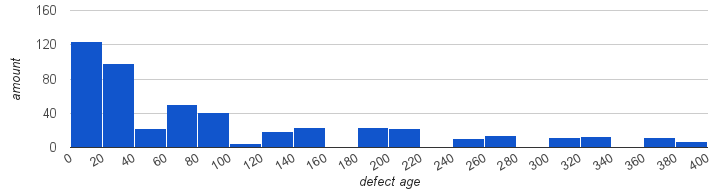
\includegraphics[width=160mm]{defect_ages.png}
\caption{Age of defects}
\end{figure}

This shows that the most common ages lays inbetween 90 to 120.
It is however important to note that defect ages doesn't directly relate to the time or effort spent on fixing bugs.
It is only a metric showing the time between when bugs have been detected and solved.
This does not imply that the bug has been worked on for so long, to retrieve this value one would have to take the difference from when a developer actually started working on fixing the bug.
%Add the diagrams comparing months and defects resolved. Defects opened might be wrong.

\subsection{Defects by component}
The number of defects per component could be used to figure out how likely it is to get defects in the different components compared to the others.
For instance the UI component quite handily has the largest number of found defects. It could be useful for figuring out where bug-fixing is most needed. But it could also mean that more testing is needed on the APT component.
However, since it doesn't show the actual code-size or complexity of the components it isn't necessarily true for similar components in other projects.
\begin{figure}[H]
\center
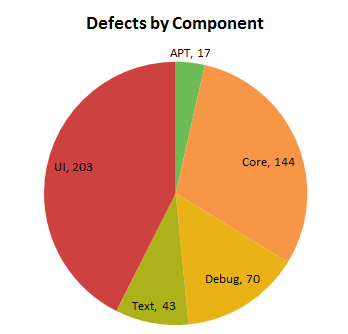
\includegraphics[width=100mm]{defects_by_component.png}
\caption{Number of defects by component}
\end{figure}

\subsection{Severe defects by component}
The severe defects of the various components could help you figure out where they are most likely to happen.
However like in the previous defects by component we do not know how large the various components are which makes it less useful for our own project, unless we were to create a similar diagram of our own defects.

\begin{figure}[H]
\center
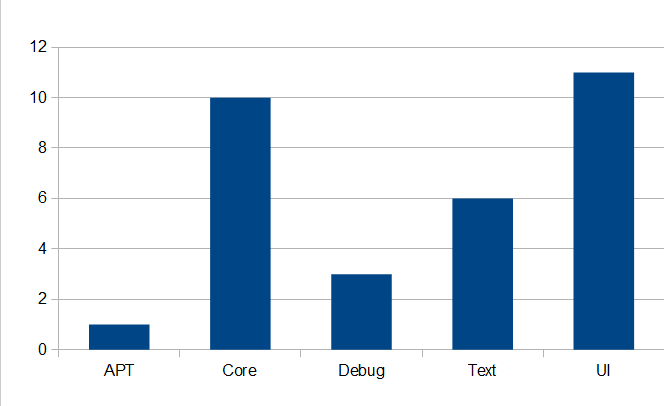
\includegraphics[width=100mm]{severe_defects_per_component.png}
\caption{Number of severe defects by component}
\end{figure}

Something we can get out of the two diagrams however, is the number of severe defects compared to the number of defects.
This gives an idea of where they tend to show up.
And while it probably varies depending on project it could be a useful indicator on where to be a little extra careful.
For instance while the UI component has a lot of defects, it is only a small percentage (5.4\%) of these that are actually severe.
On the other hand, while there are not that many defects in the text component almost 14\% of them are severe.
%Compare the defects and severe defects per component "defect comparison.txt" in dropbox. Mention how it could be useful for our project.
%Do the last part about other diagrams or information in the data that could be useful for our project.

\subsection{Monthly activity}
This diagram shows the number of bugs being resolved per month.
We marked the big releases (June) as yellow and the service releases green.
\begin{figure}[H]
\center
\includegraphics[width=150mm]{defects_resolved.png}
\caption{Number of bugs resolved per month}
\end{figure}
Here, the largest amount of defects was resolved in September 2011, although August is not far behind. 
Oracle have their big releases of eclipse at the end of June and it makes sense that there would be a plenty of incoming feedback after these large releases.
Also, based on the bug dataset, defects seem to only be handled for the first two weeks each month.
Many of them could therefore remain after the fixes done during July.

They also release their first service release at the end of September which means they probably work hard to get rid of as many problems as possible prior to that.
It is interesting however that prior to the second service release there is not an increase in resolved defects, but rather the other way around. 
The defects fixed here might have taken more time.

Now, if we instead take a look at the number of opened bugs per month, we see a clearer pattern.
\begin{figure}[H]
\center
\includegraphics[width=150mm]{defects_opened.png}
\caption{Number of bugs opened per month}
\end{figure}
Not only does it conclude with previous points (there are generally less bugs opened after service releases than before), but this diagram implies a slow decrease of the dataset as a whole.
This implies that eclipse has gotten more and more stable over time.
Most likely a lot of more unit tests have been written with increased code and use case-coverage to make the occurrence of completely new bugs less likely.
By automating testing, bugs can instead be found before commits and often even solved, which makes filing them redundant.

Next is the question about the first 3 months and their oddity.
During the first months, there were very few bugs being filed and none of them resolved.
For this we see two possibilities.
First is the fact that the bug data only goes as far back as to when the eclipse project started to use bugzilla.
Hence, it may have taken a while to get people into actually using the system; the first filed bugs might even have been for testing or as examples for employees.
There is also the chance that a core change was done prior to January that produced a lot of transitive chain reactions of bugs.
There were no big final release prior to January, however the change could either have been included in some beta version or all bugs where filed from developers. 
The change could also have been on some external system having large impact on eclipse.

One might question if it's really a good thing that less bugs are being discovered.
For eclipse however, the users have been large contributors to bug discovering, and as previously stated in \ref{user based testing} "If the customer(s) thinks the software works, it works.�

%\url{http://wiki.eclipse.org/Simultaneous_Release}

\end{document}
